% (C) 2016 Jean Nassar. Some Rights Reserved
% Except where otherwise noted, this work is licensed under the Creative Commons Attribution-ShareAlike License, version 4
% SPIRIT
\chapter{Proposal}
\label{sec:proposal}
% \setlength{\epigraphwidth}{0.43\textwidth}
%\epigraphhead{\epigraph{
  %If you don't know where you are, then you don't know where you're going.
%}{\emph{I Shall Wear Midnight}\\\textsc{Terry Pratchett}}}
  The proposal was to upgrade \gls{spir} to allow it to work better with quadrotors.
  Operator workload should decrease in positioning and orientation tasks.

  A framework should be built which would allow the modular implementation of the core functions of \gls{spir}:

  \begin{enumerate}
    \item Obtain the robot position by the best method for each robot.
    \item Save images obtained by the camera, and the pose and time at which they were taken.
    \item Select the best frame according to an evaluation function.
          That robot should ideally be seen from a good position and orientation with respect to the rest of the environment.
    \item Generate and display the rendering of the current robot position onto the selected frame.
  \end{enumerate}

  The system was built in \gls{ros} for interoperability and future expansion, as well as its ease of modularization.

  \begin{figure}[h]
    \centering
    \begin{subfigure}[b]{0.45\textwidth}
      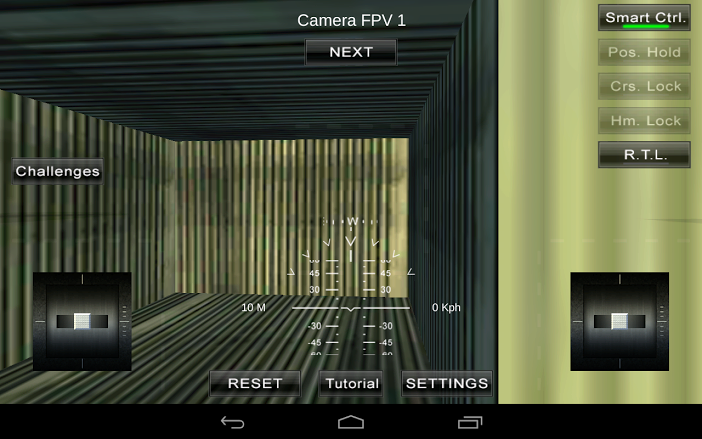
\includegraphics[width=\textwidth]{drone_sim_fpv}
      \caption{First-person View.}
    \end{subfigure}
    \hfill
    \begin{subfigure}[b]{0.45\textwidth}
      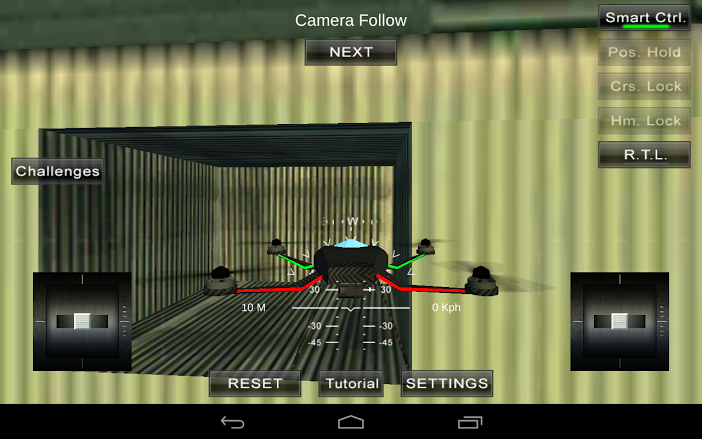
\includegraphics[width=\textwidth]{drone_sim_chase}
      \caption{External view.}
    \end{subfigure}
    \caption[Difference between FPV and external views]{The difference between \gls{fpv} and an external view. These screenshots are taken from the QuatcopterFX Simulator app on Android.}
    \label{fig:fpv_vs_chase}
  \end{figure}

  The actual implementation is discussed below.

\chapter{System overview}
  The system overview for \gls{spirit} is shown in \fref{fig:spirit_flowchart}.

  \begin{figure}[h]
    \centering
    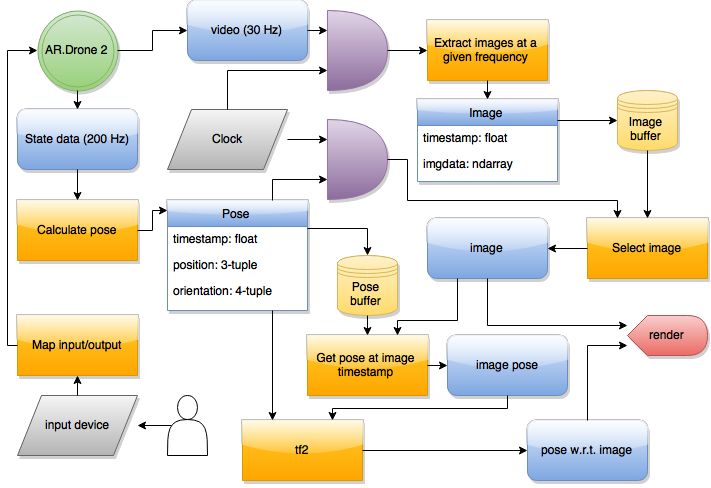
\includegraphics[width=0.9\textwidth]{spirit_flowchart}
    \caption[SPIRIT system overview]{\gls{spirit} system overview.}
    \label{fig:spirit_flowchart}
  \end{figure}

  There are six main parts to the project:

  \begin{itemize}
    \item An operator-controlled gamepad sends commands to the \gls{ardrone}.
    \item The pose, consisting of the position and orientation of the drone, is calculated by a commercial motion capture system and relayed to the operating station.
    \item The drone streams video at 30\,Hz, which is downsampled to 2\,Hz to simulate \gls{los} conditions.
    \item The 2\,Hz video feed is shown to the operator without modification.
    \item All received images are also stored in a chronological array.
	  When a new pose is received, it is checked against all frames using an evaluation function.
    \item The frame with the lowest score is selected, and has the current pose rendered onto it to show to the operator.
  \end{itemize}

\chapter{General components}
  \section{Environment}
    The operating station runs in a single \gls{docker} container on a Linux laptop.
    The primary components of the \gls{docker} image are:

    \begin{itemize}
      \item \gls{ros}
      \item Python 2.7
      \item Virtualenv
      \item \gls{opengl}
      \item Nvidia drivers
      \item Necessary \gls{ros} and Python packages
    \end{itemize}

    A separate Windows laptop has separate ethernet connections to the lab's motion capture system and to the operating station.
    The \gls{ardrone} connects to the operating station by acting as a Wifi access point.
    Communication with the drone is achieved using the \textsf{\detokenize{ardrone_autonomy}} package from Simon Fraser University's Autonomy Laboratory.

    The research code was written entirely in Python.
    Taking advantage of \gls{ros}'s modularity, each function is completely encapsulated in one or more nodes.
    As a result, implementing a new algorithm or introducing a new method to obtain data simply involves writing new code which publishes to the correct nodes.
    Any supported programming languages can be used.
    For instance, the speed of \cpp\ can be leveraged where necessary.
    
    In addition, launch files are generated on the fly from \textsf{xacro} files, with configuration data stored in various \gls{yaml} files.
    Selecting and changing coefficients of the various evaluation functions, for example, is in the \textsf{\detokenize{launch_config.yaml}} file.
    The configuration generator inspects the source code to ensure that the evaluation function class exists and that each component is indeed a runnable method.
    The generator also sets the default values of various parameters, such as the \gls{ardrone}'s \gls{ip} address or the device file for the controller.
    Identifying the controllers and selecting the correct mapping has also been demonstrated, but is not implemented in the final setup.
    % TODO: Has it been implemented yet?

    The \gls{ros} graph is shown in \fref{fig:rqt_graph}.
    % TODO: Add rqt_graph.
    \begin{figure}[h]
      \centering
      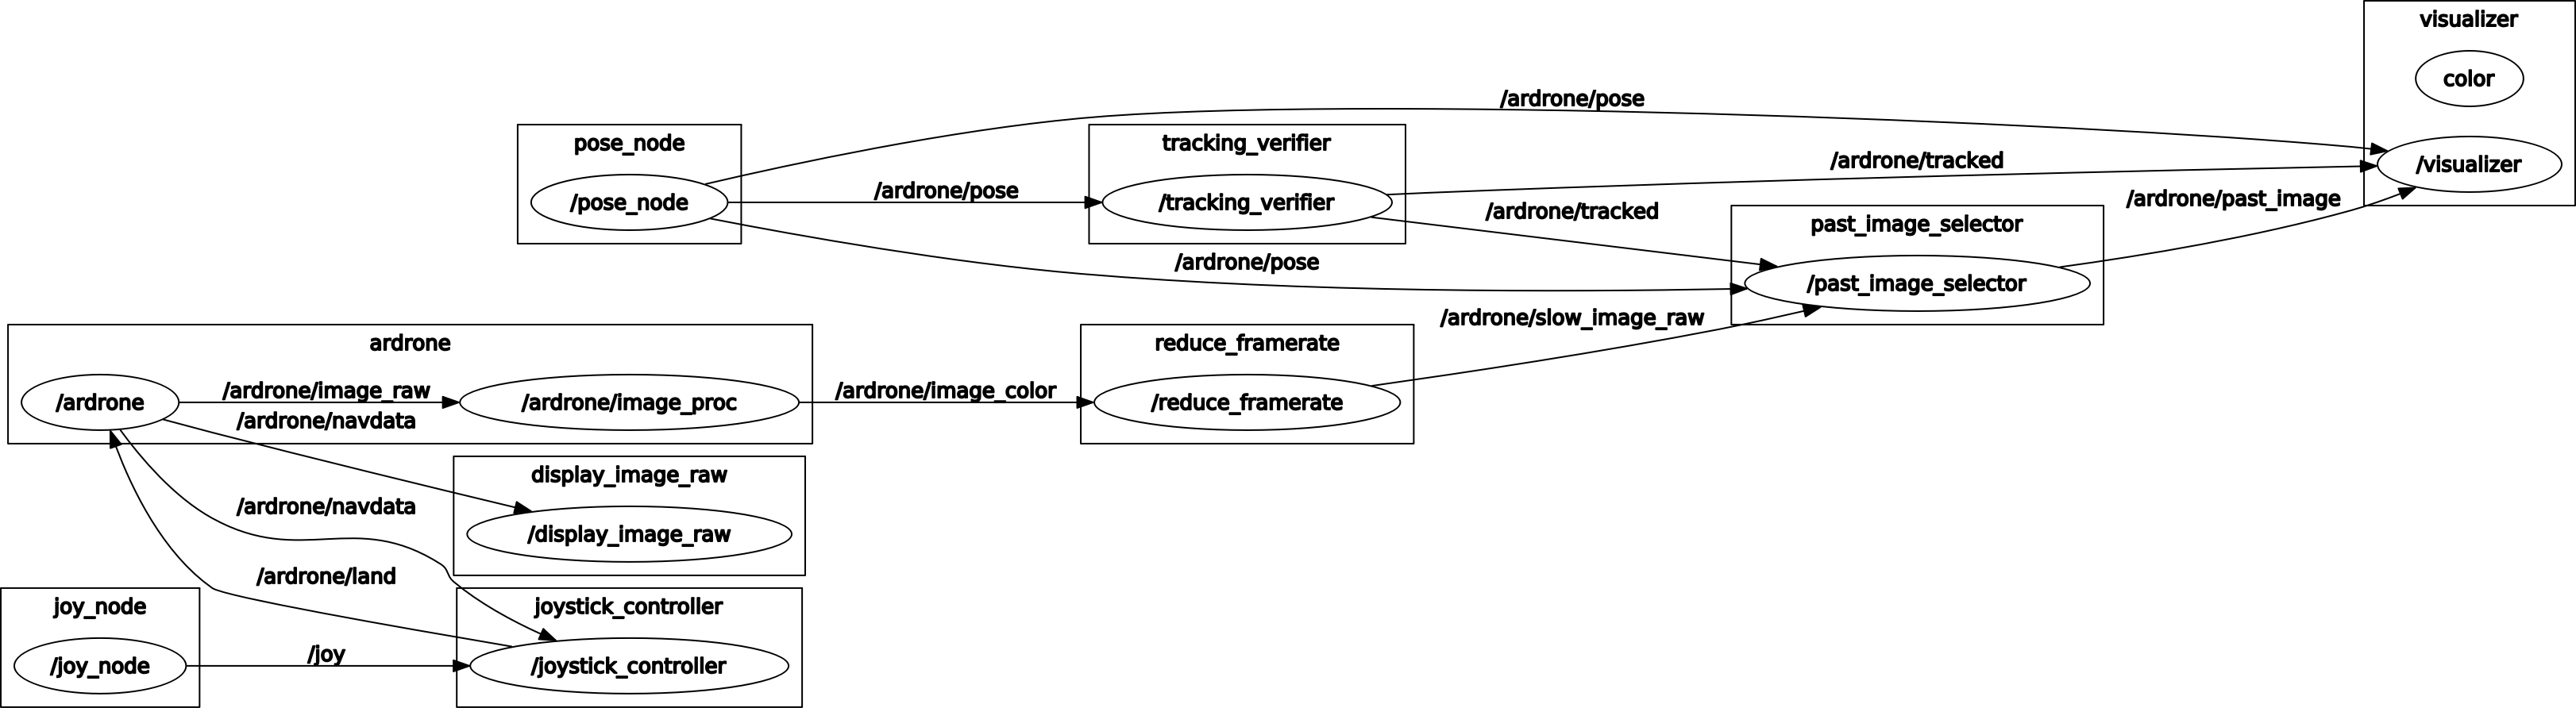
\includegraphics[width=\textwidth]{rqt_graph}
      \caption[ROS Graph]{The \gls{ros} graph for the system.}
      \label{fig:rqt_graph}
    \end{figure}

  \section{Control}
    The operating station receives operator input from an off-the-shelf \gls{ps3} console gamepad, and forwards it to the drone.
    After the setup of the button and axis mappings was complete, the controller publishes directly to the relevant \texttt{\detokenize{/ardrone}} nodes set up by \textsf{\detokenize{ardrone_autonomy}}.

    There is no automation in flying the \gls{ardrone} apart from the built-in \gls{ai}.
    The default control system implemented by Parrot is used.

  \section{Video}
    A live 30\,Hz feed is received from the drone.
    In order to simulate \gls{los} conditions, the feed frequency was dropped to 2\,Hz by only selecting every fifteenth frame.

    The slower feed is republished for other nodes.
    Specifically, its frames are the ones stored in the buffer used in selecting past images, and the video was also displayed to the user for increased situational awareness.

  \section{Abstractions}
    \gls{ros}'s \texttt{PoseStamped} messages are wrapped as a \texttt{Pose} object, which exposes the position and orientation of the message as numpy arrays.
    This class also allows the calculation of relative Euler angles and distances with other \texttt{Pose}s.

    New \texttt{Image}s (from \textsf{\detokenize{sensor_msgs.msg}}) and the latest available \texttt{Pose} are stored in a \texttt{Frame} object.
    A \texttt{Frame} also allows easy calculation the relative position with another \texttt{Pose} in the local reference frame.
    Since the same calculation is run multiple times per frame, the result was memoized, causing a significant speedup.
  

\chapter{Poses}
\label{sec:poses}
  \section{Terminology}
    Roll (\sym{roll}), pitch (\sym{pitch}), and yaw (\sym{yaw}) refer to rotations about the respective axes (\sym{rollaxis}, \sym{pitchaxis}, \sym{yawaxis}), as shown in \fref{fig:drone_rpy}.
    The convention used in this report are with respect to the body frame of reference. The positive direction is determined by the right-hand rule.

    \begin{figure}[h]
      \centering
      \begin{subfigure}[b]{0.45\textwidth}
	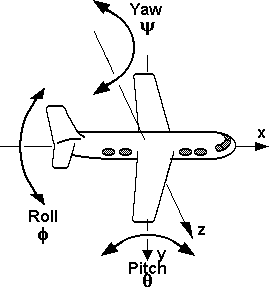
\includegraphics[width=\textwidth]{drone_rpy}
	\caption{Roll, pitch, and yaw.}
	\label{fig:drone_rpy}
      \end{subfigure}
      \hfill
      \begin{subfigure}[b]{0.45\textwidth}
	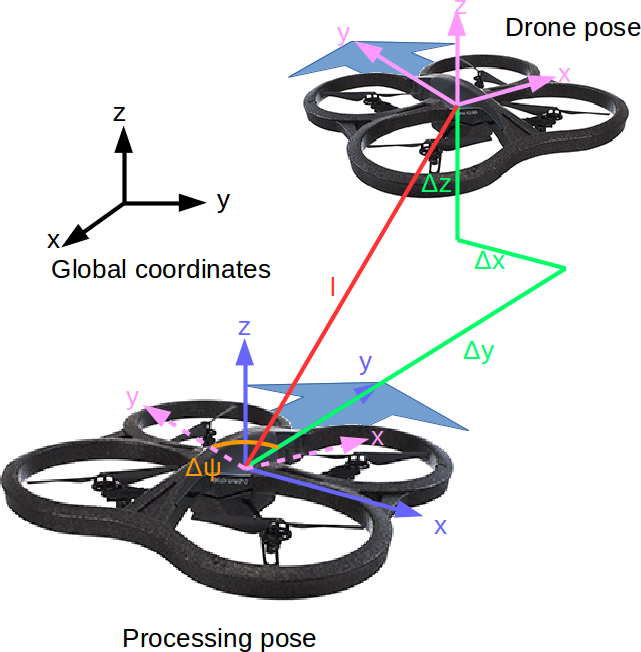
\includegraphics[width=\textwidth]{drones_ref}
	\caption{Pose variables.}
	\label{fig:drones_ref}
      \end{subfigure}
      \caption[Pose parameter definitions]{\fref{fig:drone_rpy} shows the definitions of roll, pitch, and yaw with respect to an aircraft in the body frame of reference. \fref{fig:drones_ref} shows the pose variables, and the relative positions of the current drone position and the frame being processed.}
    \end{figure}

    The position of the drone is represented by \sym{pos}, and defined as:

    \begin{equation}
      \sym{pos} = \begin{bmatrix}
	\sym{posx} \\
	\sym{posy} \\
	\sym{posz} \\
      \end{bmatrix}
    \end{equation}

    where \sym{posx}, \sym{posy}, and \sym{posz} are the $x$, $y$, and $z$ components.

    The orientation of the drone is represented by a quaternion, \sym{quat}, and defined as:

    \begin{equation}
      \sym{quat} = \begin{bmatrix}
	\sym{quatx} \\
	\sym{quaty} \\
	\sym{quatz} \\
	\sym{quatw} \\
      \end{bmatrix}
    \end{equation}

    such that the quaternion can also be represented as $\sym{quatw} + \sym{quatx}\mathbf{i} + \sym{quaty}\mathbf{j} + \sym{quatz}\mathbf{k}$.
    $\mathbf{i}$, $\mathbf{j}$, and $\mathbf{k}$ are the basis elements of the quaternion, and they are related by:

    \begin{equation}
      \mathbf{i}^2 = \mathbf{j}^2 = \mathbf{k}^2 = \mathbf{ijk} = -1
    \end{equation}

    The state vector is $\sym{state} = \begin{bmatrix}\sym{pos} & \sym{quat}\end{bmatrix}^\top$.
    
    The rotation matrix \sym{rotmat}, based on quaternions, is defined as:\cite{wiki_rotmat}

    \begin{equation}
      \sym{rotmat} = \begin{bmatrix}
	1 - 2\sym{quaty}^2 - 2\sym{quatz}^2 & 2\sym{quatx}\sym{quaty} - 2\sym{quatz}\sym{quatw} & 2\sym{quatx}\sym{quatz} + 2\sym{quaty}\sym{quatw} \\
	2\sym{quatx}\sym{quaty} + 2\sym{quatz}\sym{quatw} & 1 - 2\sym{quatx}^2 - 2\sym{quatz}^2 & 2\sym{quaty}\sym{quatz} - 2\sym{quatx}\sym{quatw} \\
	2\sym{quatx}\sym{quatz} - 2\sym{quaty}\sym{quatw} & 2\sym{quaty}\sym{quatz} + 2\sym{quatx}\sym{quatw} & 1 - 2\sym{quatx}^2 - 2\sym{quaty}^2
      \end{bmatrix}
    \end{equation}

    Finally, \sym{rfcurrent}, \sym{rfdrone}, \sym{rfprocessed}, and \sym{rfglobal} are the reference frames of the currently displayed frame, the drone, the frame being processed, and the global coordinate system respectively.

  \section{Relative poses}
    \subsection{Relative position}
    In order to find the relative position of the drone with respect to the frame being processed, the orientation of the frame must first be cancelled out by the rotation matrix.
    
    \begin{equation}
      ^{\sym{rfprocessed}}_{\sym{rfdrone}}\Delta\sym{pos} = 
      ^{\sym{rfglobal}}_{\sym{rfprocessed}}\sym{rotmat}\left(\sym{pos}_{\sym{rfdrone}} - \sym{pos}_{\sym{rfprocessed}}\right) = 
      \begin{bmatrix}
	\Delta\sym{posx} \\
        \Delta\sym{posy} \\
        \Delta\sym{posz}
      \end{bmatrix}_{\sym{rfprocessed}\sym{rfdrone}}
    \end{equation}

    \subsection{Relative orientation}
    In order to find the relative orientation of the drone with respect to the frame being processed, we need to find the quaternion product.

    \begin{equation}
      ^{\sym{rfprocessed}}_{\sym{rfdrone}}\Delta\sym{quat} = \hat{\sym{quat}}_{\sym{rfprocessed}}\hat{\sym{quat}}_{\sym{rfdrone}}
    \end{equation}

    First, set the imaginary components of the quaternion to \sym{quatim} such that:

    \begin{equation}
      \sym{quatim} = \begin{bmatrix}\sym{quatx} \\ \sym{quaty} \\ \sym{quatz}\end{bmatrix}
    \end{equation}

    and $\sym{quat} = \begin{bmatrix}\sym{quatim} & \sym{quatw}\end{bmatrix}^\top$. The solution is:

    \begin{equation}
      ^{\sym{rfprocessed}}_{\sym{rfdrone}}\Delta\sym{quat} = \begin{bmatrix}
	\sym{quatw}_{\sym{rfprocessed}}\sym{quatim}_{\sym{rfdrone}} + \sym{quatw}_{\sym{rfdrone}}\sym{quatim}_{\sym{rfprocessed}} + \sym{quatim}_{\sym{rfprocessed}}\times\sym{quatim}_{\sym{rfdrone}} \\
	\sym{quatw}_{\sym{rfprocessed}}\sym{quatw}_{\sym{rfdrone}} - \sym{quatim}_{\sym{rfprocessed}}\cdot\sym{quatim}_{\sym{rfdrone}}
      \end{bmatrix}
    \end{equation}
    

  \section{Motion capture}
    Optitrack's \emph{Motive} software is used to collect \gls{mocap} data on the position and orientation of the drone.
    Four infrared markers are set onto the top of the drone, and the Optitrack infrared cameras are connected to the \gls{mocap} computer.
    The markers forming the drone are defined as a rigid body, allowing the pose information to be calculated for the entire drone at once.

    % TODO: Mocap screenshots.

    The \gls{mocap} system then streams the data, including the rigid body information, via multicast.
    The data is received by the operating station, interpreted by \gls{ros}'s \textsf{\detokenize{mocap_optitrack}} package, and republished to \texttt{/ardrone}'s \texttt{\detokenize{pose}} and \texttt{\detokenize{ground_pose}} nodes.
    The latter uses quaternions instead of the Eulerian coordinates which \emph{Motive} displays.

    The motion capture setup was good for prototyping without needing to turn on the drone, and it had good accuracy compared to, say, \gls{gps}.
    However, depending on it led to an extremely limited usage area, since the drone had to be within range of multiple \gls{mocap} cameras.

    If the \gls{mocap} system is unable to determine the pose of the drone, whether by marker occlusion or lack of information, \emph{Motive} sends the last known position instead of raising an error.
    In that case, the visualization system would be using out-of-date pose data, which could cause problems.
    As a result, the pose is tracked over time, and the boolean status is published to \texttt{\detokenize{/ardrone/tracked}} and can be used by other nodes.
    For instance, if tracking is lost, an audible horn sounds, accompanied by a visual warning for the operator, as shown in \fref{fig:spirit_interface_lost}.

    \begin{figure}[h]
      \centering
      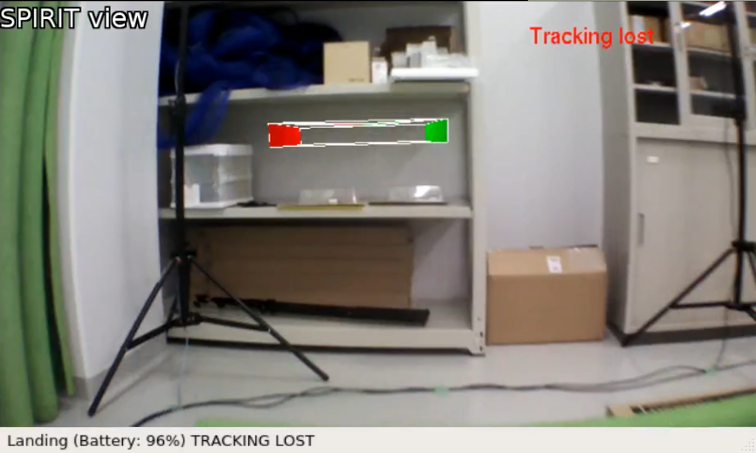
\includegraphics[width=\textwidth]{spirit_interface_lost}
      \caption[Interface with tracking lost]{A screenshot of the \gls{spirit} interface when tracking has been lost. Notice the red text in the upper-right corner. The operator can still see the 2\,Hz live feed.}
      \label{fig:spirit_interface_lost}
    \end{figure}

  \section{Other methods}
    One method of obtaining the pose, which is not used in the final setup, is the ability of \textsf{\detokenize{ardrone_autonomy}} to obtain drone odometry from the bottom-facing camera, \gls{imu}, altimiter, and barometer.
    The ground velocity is calculated using integration of the acceleration as well as optical flow.
    While the final result proved to be accurate, the calculations required were too slow in a tight loop when running on the operating station.
    Therefore, it was discarded in favour of the motion capture system.

\chapter{Selection of past images}
    Each new image that arrives while the pose is being tracked is automatically packaged into a \texttt{Frame} object containing the time it was taken, as well as the position and orientation of the drone at that time.
    These \texttt{Frame}s are then stored in a chronological list, which is implemented as a deque.

    When a new valid pose arrives, it is checked against the frames using an evaluation function.
    The \texttt{Frame} with the lowest score is published for use by the visualization system.

    However, while the pose was sampled at 200\,Hz (every 5\,ms), each iteration of some of the evaluation functions requires up to 0.3\,ms to run.
    As a result, when about twenty frames are collected, a substantial lag in image selection can be detected.
    To mitigate this, when a new frame is still in the process of being selected, the visualizer displays the new pose on the currently shown frame.

    The maximum queue length can be set in the launch parameter configuration file.
    The final setup used a maximum of 60\,frames, or 30\,s of video.
    This allows each loop to run its course before the next pose is received.

  \section{Evaluation functions}
    In this section, all $\Delta$ differences are from the drone with respect to the frame being processed, unless otherwise specified.
    In addition, $_{ref}$ indicates a reference, or ideal value, which can be set by the operator.
    \fref{fig:drones_view} shows the relative positions. For more information on the notation, please see Section \ref{sec:poses}.

    \begin{figure}[h]
      \centering
      \begin{subfigure}[b]{0.45\textwidth}
	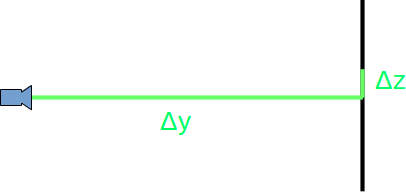
\includegraphics[width=\textwidth]{drones_view_side}
	\caption{From the side.}
      \end{subfigure}
      \hfill
      \begin{subfigure}[b]{0.45\textwidth}
	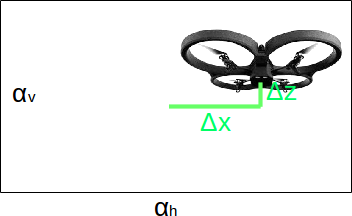
\includegraphics[width=\textwidth]{drones_view_front}
	\caption{From the front.}
      \end{subfigure}
      \caption[Relative positions]{The relative position of the drone with respect to the frame being processed, in terms of camera positioning.}
      \label{fig:drones_view}
    \end{figure}

    Evaluation functions are defined as:

    \begin{equation}
      \sym{evalfn} = \sum_{\sym{elemidx}=1}^{\sym{nelems}}{\sym{coeff}_{\sym{elemidx}}\sym{elem}_{\sym{elemidx}}}
    \end{equation}
    
    where $\sym{nelems}$ is the number of elements in the evaluation function, $\sym{elem}_{\sym{elemidx}}$ is an element, and $\sym{coeff}_{\sym{elemidx}}$ is its corresponding coefficient.
    After evaluation, the frame with the lowest score is selected, and its contents are streamed to the \texttt{/ardrone} namespace's \texttt{\detokenize{past_image}} and \texttt{\detokenize{past_pose}} nodes.

    \subsection{Naïve evaluation functions}
      The simplest evaluation function for past image view is one with constant time delay, as suggested by Shiroma et al.\cite{shiroma2004}
      One can quickly find a frame with a specific age by doing a binary search in the chronologically-ordered array.
      However, while it works well for robots moving at a relatively constant velocity with minimal direction change, it does not track sudden movements, accelerations, or stoppages.

      On the other hand, Shiroma et al.'s constant distance evaluation function\cite{shiroma2004} maintains the distance effectively, and works well with robots which change their orientation gradually.
      With a drone, though, the operator can move in any direction at any time, including backwards, and the selected frame might not contain the drone's current position at all.

      Note that both these evaluation functions have also been implemented, and are accessible by setting the appropriate value in the \texttt{\detokenize{launch_config.yaml}} file.

    \subsection{Murata evaluation function}
      Murata et al.'s evaluation function was designed for \gls{3d} environments,\cite{murata2014} and an attempt was made at using it.

      The evaluation function is:

      \begin{equation}
	\begin{split}
	  \sym{evalfn}_{\mathrm{Murata}}
	               &= \sym{coeff}_1\left(\frac{\Delta\sym{posz} - \Delta\sym{posz}_{ref}}{\Delta\sym{posz}_{ref}}\right)^2  % relative height
		        + \sym{coeff}_2\left(\frac{2\Delta\sym{yaw}}{\pi}\right)^2  % pointing in the same direction
	                + \sym{coeff}_3\left(\frac{\arctan\left(\frac{\sqrt{\Delta\sym{posx}^2 + \Delta\sym{posz}^2}}{\Delta\sym{posy}}\right)}{\sym{aovv}}\right)^2 \\  % tilt angle
	               &+ \sym{coeff}_4\left(\frac{\left\|\Delta\sym{pos}\right\| - \left\|\Delta\sym{pos}\right\|_{ref}}{\left\|\Delta\sym{pos}\right\|_{ref}}\right)^2   % distance
	                + \sym{coeff}_5\left(\frac{\left\|\sym{state}_{\sym{rfprocessed}} - \sym{state}_{\sym{rfcurrent}}\right\|}{\sym{state}_{\sym{rfcurrent}}}\right)^2  % minimize change
	\end{split}
      \end{equation}

      where \sym{aovv} is the vertical angle of view such that:

      \begin{equation}
	\sym{aovv} = 2\arctan\left(\sym{aovr}\tan\frac{\sym{aovh}}{2}\right)
      \end{equation}

      where \sym{aovr} is the aspect ratio of the display and \sym{aovh} is the horizontal angle of view.

      The five components are as follows:

      \begin{itemize}
	\item $\sym{elem}_1$ represents the height of the viewpoint.
	      We want to see the drone from slightly above.
	\item $\sym{elem}_2$ represents the azimuth angle of the viewpoint.
	      We want to see the drone from behind.
	\item $\sym{elem}_3$ represents the tilt angle of the viewpoint.
	      The closer it is to zero, the closer to the centre of the image the drone is.
	\item $\sym{elem}_4$ represents the distance to the drone.
	      We want to be as close as possible to an ideal distance away, such that the drone is neither too big nor too small.
	\item $\sym{elem}_5$ represents the movement of the viewpoint if the frame being processed is selected.
	      The smaller it is, the smoother the transition.
      \end{itemize}

      Murata et al.'s function performed much better than the naïve ones.
      However, actual usage indicated that there was a bad performance in high speed environments and in tight turns.

      The values of the coefficients as used while evaluating the Murata et al. function are shown in Table \ref{tab:murata_coeffs}.

      % TODO: Update final values.
      \begin{table}[h]
	\centering
	\caption[Murata coefficient values]{The values of the coefficients used for Murata et al.'s function.}
	\begin{tabular}{ll}
	  \toprule
	  Coefficient & Value \\
	  \midrule
	  $\sym{coeff}_1$ & 2 \\
	  $\sym{coeff}_2$ & 0.4 \\
	  $\sym{coeff}_3$ & 0.8 \\
	  $\sym{coeff}_4$ & 4 \\
	  $\sym{coeff}_5$ & 0 \\
	  \bottomrule
	\end{tabular}
	\label{tab:murata_coeffs}
      \end{table}

      The reference height and distance were set to 0.3 and 1.5\,m respectively.

    \subsection{SPIRIT evaluation function}
      The final version of the \gls{spirit} evaluation function is:

      \begin{equation}
	\begin{split}
	  \sym{evalfn}_{\mathrm{\gls{spirit}}}
	               &= \sym{coeff}_1\frac{\sqrt{\Delta\sym{posx}^2 + \Delta\sym{posz}^2}}{\left\|\Delta\sym{pos}\right\|_{ref}}  % centrality
			+ \sym{coeff}_2\Delta\sym{yaw}^2  % relative yaw
	                + \sym{coeff}_3\left(\frac{\left\|\Delta\sym{pos}\right\| - \left\|\Delta\sym{pos}\right\|_{ref}}{\left\|\Delta\sym{pos}\right\|_{ref}}\right)^2 \\  % distance
		       &+ \sym{coeff}_4{}^{\sym{rfcurrent}}_{\sym{rfprocessed}}\Delta\sym{yaw}^2  % frame direction
			+ \sym{coeff}_5\frac{\left\|^{\sym{rfcurrent}}_{\sym{rfprocessed}}\Delta\sym{pos}\right\|}{\left\|\Delta\sym{pos}\right\|_{ref}}  % frame distance
	\end{split}
      \end{equation}

      The five components are as follows:

      \begin{itemize}
	\item $\sym{elem}_1$ represents the centrality, or how close the drone is to the centre of the frame.
	\item $\sym{elem}_2$ represents the difference in yaw between the drone and the frame.
	      We would like to see the drone directly from behind, and face in the same direction as it.
	\item $\sym{elem}_3$ represents the distance to the drone.
	      We want to be as close as possible to an ideal distance away, such that the drone is neither too big nor too small.
	\item $\sym{elem}_4$ represents the difference in yaw between the currently displayed frame and the frame being processed.
	      The smaller it is, the smaller the angular difference is if the frame is selected.
	\item $\sym{elem}_5$ represents the difference in distance between the currently displayed frame and the frame being processed.
	      The smaller it is, the closer the two frames are and the smoother the transition.
      \end{itemize}

      A previous version of $\sym{elem}_1$, centrality, was:

      \begin{equation}
	\sym{elem}_{1,\mathrm{old}} = \frac{\Delta\sym{posx}^2 + \Delta\sym{posz}^2}{\Delta\sym{posy}^2}
      \end{equation}

      However, it was not used in the final setup because $\sym{elem}_1$ was more effective.  % TODO: Was it?

      % TODO: Talk about problems with some coefficients?
      Brute-forcing was used to find a range of relative stability for the coefficients, where quick changes of the displayed past image were minimized.
      After that, experimentation was used to select ones which provided a good experience.  

      The values of the coefficients as used in the experiments are shown in Table \ref{tab:coeffs} below.

      % TODO: Update final values.
      \begin{table}[h]
	\centering
	\caption[Final coefficient values]{The values of the coefficients used in the user experiments.}
	\begin{tabular}{ll}
	  \toprule
	  Coefficient & Value \\
	  \midrule
	  $\sym{coeff}_1$ & 8 \\
	  $\sym{coeff}_2$ & 4 \\
	  $\sym{coeff}_3$ & 8 \\
	  $\sym{coeff}_4$ & 1 \\
	  $\sym{coeff}_5$ & 2 \\
	  \bottomrule
	\end{tabular}
	\label{tab:coeffs}
      \end{table}

      In addition, the reference distance was set to 3\,m.
      The thresholds for distance and yaw, below which a new frame is not selected, were set to 10\,cm and 5 degrees respectively.

\chapter{Visualization}
  Visualization in \gls{ros} is usually done with \gls{rviz}.
  However, due to a lack of good documentation during the early implementation phase, as well as various problems in displaying the background correctly with respect to the drone avatar, it was abandoned for a custom solution.
  The most advanced state with \gls{rviz} is shown in \fref{fig:rviz_display}.

  \begin{figure}[h]
    \centering
    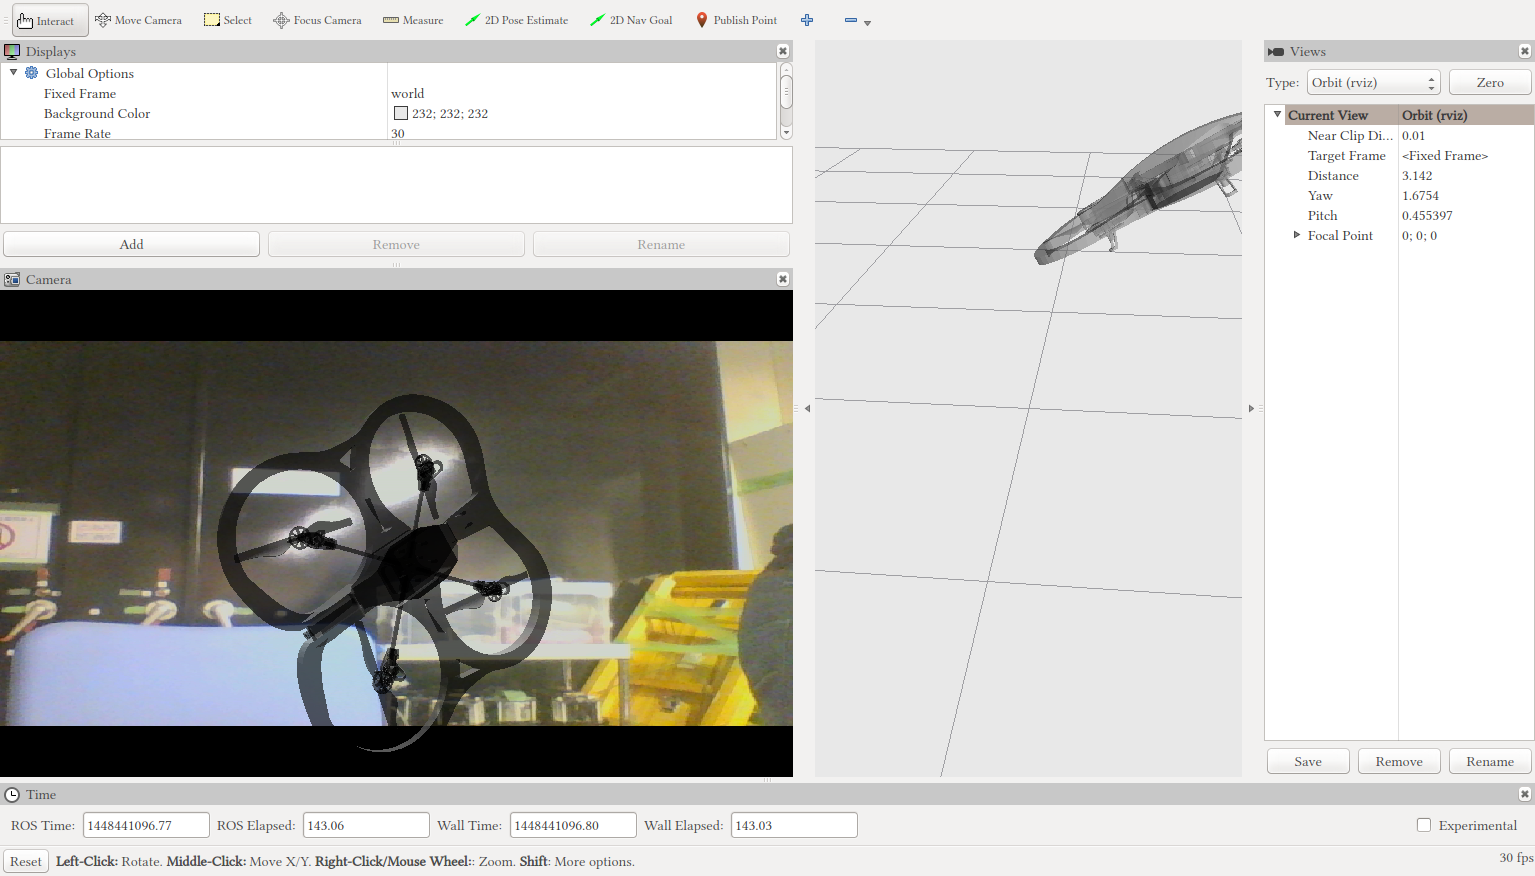
\includegraphics[width=\textwidth]{rviz_display}
    \caption[rviz maximum progress]{Maximum progress with \gls{rviz}.}
    \label{fig:rviz_display}
  \end{figure}

  \section{Components}
    Visualization in this project uses three different libraries: \gls{pyopengl}, \gls{pygame}, and \gls{pyqt5}.

    \subsection{PyOpenGL}
    \gls{pyopengl} is used to render the avatar of the \gls{ardrone} in the scene.
    The current drone pose information is in the \texttt{/ardrone/pose} node, while the frame information is obtained from the \texttt{\detokenize{past_image}} and \texttt{\detokenize{past_pose}} nodes of the same namespace.

    Context managers for commonly-used \gls{pyopengl} functionality were written to ease development.
    
    \subsection{Pygame}
    \gls{pygame} is used to produce the horn sounds if tracking is lost or reacquired.
    It is also used to host the \gls{pyopengl} scene which is rendered.
    However, simple tasks require a roundabout way of doing things, so future iterations may not use \gls{pygame} at all.

    \subsection{PyQt5}
    \gls{pyqt5} is used to create a window for streaming video feeds.
    When the \gls{ardrone} is connected, its remaining battery percentage and flight status are displayed in the status bar at the bottom of the window.
    % TODO: show PyQT5 window screenshot.

    \gls{pyqt5} could also be used to replace \gls{pygame} for producing the horn sound when tracking is lost or reconnected, as well as hosting the \gls{pyopengl} scene.
    At the time of writing, this is yet to be done.

  \section{Rendering}
    The visualizer is run as a multithreaded application in order to maximize responsiveness.
    After obtaining the relevant data, the relative positions and orientations of the drone and the frame are calculated.
    A new texture is automatically loaded whenever a new \texttt{\detokenize{past_image}} is published, and is used as the frame when the scene is rendered.

    \gls{opengl} uses an axis-angle representation, so the relative orientation is converted from quaternion to axis angle using the following formula:

    \begin{align}
      \sym{rotang} &= 2\arccos\sym{quatw} \\
      \sym{uvec} &= 
      \begin{dcases}
	\begin{bmatrix}1 & 0 & 0\end{bmatrix},& \text{if } \sym{rotang} = 0 \\
	\begin{bmatrix}\sym{quatx} & \sym{quaty} & \sym{quatz}\end{bmatrix},& \text{if } \sym{rotang} \bmod 180 = 0 \\
      \frac{\begin{bmatrix}\sym{quatx} & \sym{quaty} & \sym{quatz}\end{bmatrix}}{\sqrt{1 - \sym{quatw}^2}} & \text{otherwise}
      \end{dcases}
    \end{align}

    where \sym{rotang} is the rotation angle.

    The scene is re-rendered whenever a new \texttt{pose} is published.
    First, the relative position is calculated as $^{\sym{rfdrone}}_{\sym{rfprocessed}}\Delta\sym{pos} = \sym{pos}_{\sym{rfprocessed}} - \sym{pos}_{\sym{rfdrone}}$, and the orientations of the frame and the drone are converted into an \gls{opengl} quaternion using the following mapping:

    \begin{equation}
      \begin{bmatrix}\sym{quatx} & \sym{quaty} & \sym{quatz} & \sym{quatw}\end{bmatrix} \mapsto
      \begin{bmatrix}-\sym{quatx} & \sym{quatz} & \sym{quaty} & \sym{quatw}\end{bmatrix}
    \end{equation}

    In a new matrix, the perspective is rotated by the same amount the frame is.
    Since the \sym{quatz} axis is with respect to the origin, not the camera, that component is first multiplied by $-1$.
    Next, the relative positions are converted to the \gls{opengl} coordinate frame using the following mapping:

    \begin{equation}
      \begin{bmatrix}\Delta\sym{posx} & \Delta\sym{posy} & \Delta\sym{posz}\end{bmatrix} \mapsto
      \begin{bmatrix}\Delta\sym{posx} & -\Delta\sym{posz} & -\Delta\sym{posy}\end{bmatrix}
    \end{equation}

    The scene translates by that amount.
    The current texture is then drawn as a \gls{2d} orthographic projection covering the entire scene.

    After that, the drone is drawn at the origin.
    The model of the drone is shown as a blank parallelipiped using \gls{opengl} primitives, with the same dimensions as the edges of the actual drone.
    A surface in the shape of an arrow is added to the top side, and coloured using the standard \gls{navlight} colouration.
    Specifically, the left side of the drone is shown in red, while its right side is in green.
    To draw it, a new matrix is pushed, and the scene is rotated by the relative orientation, after which the individual components are added.

    Finally, text can be superimposed using orthographic projection, if it is necessary.
    This is used, for instance, when warning the operator that there is no data yet, or when tracking is lost.

    The final interface is shown in \fref{fig:spirit_interface_tracked}.

    \begin{figure}[h]
      \centering
      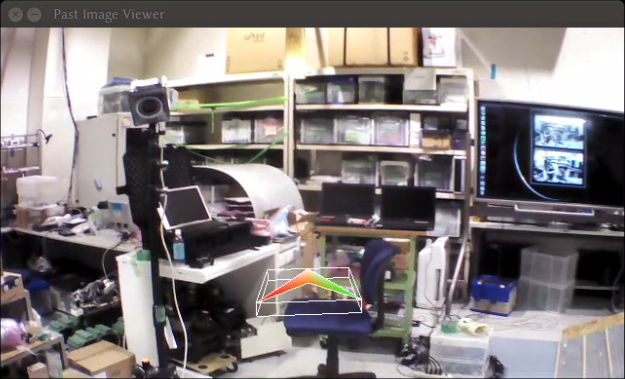
\includegraphics[width=\textwidth]{spirit_interface_tracked}
      \caption[SPIRIT final interface]{Final interface for \gls{spirit}, with the \gls{ardrone} tracked. Here, the operator is attempting to land it on a chair.}
      \label{fig:spirit_interface_tracked}
    \end{figure}
    
    An offline testing mode, with an optional web camera feed, was added to the past-image visualizer for debugging purposes.

    % TODO: Full screnshot of UI.
